\documentclass[11pt,twoside=off,numbers=noenddot]{scrbook}

%%fakesection Load packages

\usepackage{lmodern}
\usepackage[pdfusetitle]{hyperref}
\ExplSyntaxOn
\sys_if_engine_luatex:T {
    \usepackage{luatex85}
}
\sys_if_engine_pdftex:T {
    \usepackage[T1]{fontenc}
}
\ExplSyntaxOff

% These are evan.sty
\usepackage{amsmath,amssymb,amsthm}
\usepackage{mathrsfs}
\usepackage[usenames,svgnames,dvipsnames]{xcolor}
\usepackage{textcomp}
\usepackage{enumerate}
\usepackage[textsize=scriptsize,shadow]{todonotes}
\usepackage{mathtools}
\usepackage{microtype}
\usepackage[normalem]{ulem}
\usepackage{stmaryrd}
\usepackage{wasysym}
\usepackage{multirow}
\usepackage{prerex}
\usepackage[nameinlink]{cleveref}

%%fakesection evan.sty macros
%Small commands
%% Napkin commands
\newcommand{\prototype}[1]{
    \emph{{\color{red} Prototypical example for this section:} #1} \par\medskip
}
\newenvironment{moral}{%
    \begin{mdframed}[linecolor=green!70!black]%
        \bfseries\color{green!50!black}}%
        {\end{mdframed}}

%%fakesection Links (hyperref loaded earlier implicitly)
\hypersetup{
    linkcolor={red!50!black},
    citecolor={green!50!black},
    urlcolor={blue!80!black},
    pdfkeywords={napkin,math},
    pdfsubject={web.evanchen.cc},
    colorlinks,
}

%%fakesection Commutative diagrams
\usepackage{tikz-cd}
\usetikzlibrary{arrows,arrows.meta}
% make a larger hook
% https://tex.stackexchange.com/questions/514451/how-to-define-a-new-hooked-arrow
\makeatletter
\pgfdeclarearrow{
    name=xGlyph,
    cache=false,
    bending mode=none,
    parameters={\tikzcd@glyph@len,\tikzcd@glyph@shorten},
    setup code={%
            \pgfarrowssettipend{\tikzcd@glyph@len\advance\pgf@x by\tikzcd@glyph@shorten}},
    defaults={
            glyph axis=axis_height,
            glyph length=+1.55ex,
            glyph shorten=+-0.1ex},
    drawing code={%
            \pgfpathrectangle{\pgfpoint{+0pt}{+-1.5ex}}{\pgfpoint{+\tikzcd@glyph@len}{+3ex}}%
            \pgfusepathqclip%
            \pgftransformxshift{+\tikzcd@glyph@len}%
            \pgftransformyshift{+-\tikzcd@glyph@axis}%
            \pgftext[right,base]{\tikzcd@glyph}}}
\makeatother
\tikzcdset{
arrow style=tikz,
diagrams={>={Latex}},
tikzcd left hook/.tip={xGlyph[glyph math command=supset, swap, glyph axis = 5.7pt]},
tikzcd right hook/.tip={xGlyph[glyph math command=supset, glyph axis = 5.7pt]},
surjective head arrow /.tip = {tikzcd to[sep=-1.5pt]tikzcd to},
surjective head/.style={
        -surjective head arrow
    }
}

%%fakesection Page layout
\usepackage[headsepline]{scrlayer-scrpage}
\renewcommand{\headfont}{}
\addtolength{\textheight}{3.14cm}
\setlength{\footskip}{0.5in}
\setlength{\headsep}{10pt}

\def\shortdate{\leavevmode\hbox{\the\year-\twodigits\month-\twodigits\day}}
\def\twodigits#1{\ifnum#1<10 0\fi\the#1}
\automark[chapter]{chapter}

\rohead{\footnotesize\thepage}
\rehead{\footnotesize \textbf{\sffamily Napkin}, by \emph{Evan Chen} (\napkinversion)}
\lehead{\footnotesize\thepage}
\lohead{\footnotesize \leftmark}
\chead{}
\rofoot{}
\refoot{}
\lefoot{}
\lofoot{}
%\cfoot{\pagemark}

%%fakesection Fancy section and chapter heads
\renewcommand*{\sectionformat}{\color{purple}\S\thesection\autodot\enskip}
\renewcommand*{\subsectionformat}{\color{purple}\S\thesubsection\autodot\enskip}
\newcommand{\problemhead}{A few harder problems to think about}
\renewcommand{\thesubsection}{\thesection.\roman{subsection}}

\addtokomafont{chapterprefix}{\raggedleft}
\RedeclareSectionCommand[beforeskip=0.5em]{chapter}
\renewcommand*{\chapterformat}{%
    \mbox{\scalebox{1.5}{\chapappifchapterprefix{\nobreakspace}}%
        \scalebox{2.718}{\color{purple}\thechapter\autodot}\enskip}}

\addtokomafont{partprefix}{\rmfamily}
\renewcommand*{\partformat}{\color{purple}\scalebox{2.5}{\thepart}}

%%fakesection Theorems
\usepackage{thmtools}
\usepackage[framemethod=TikZ]{mdframed}

\theoremstyle{definition}
\mdfdefinestyle{mdbluebox}{%
    linewidth=1pt,
    skipabove=12pt,
    innerbottommargin=9pt,
    skipbelow=2pt,
    nobreak=true,
    linecolor=blue,
    backgroundcolor=TealBlue!5,
}
\declaretheoremstyle[
    headfont=\sffamily\bfseries\color{MidnightBlue},
    mdframed={style=mdbluebox},
    headpunct={\\[3pt]},
    postheadspace={0pt}
]{thmbluebox}

\mdfdefinestyle{mdredbox}{%
    linewidth=0.5pt,
    skipabove=12pt,
    frametitleaboveskip=5pt,
    frametitlebelowskip=0pt,
    skipbelow=2pt,
    frametitlefont=\bfseries,
    innertopmargin=4pt,
    innerbottommargin=8pt,
    linecolor=RawSienna,
    backgroundcolor=Salmon!5,
}
\declaretheoremstyle[
    headfont=\bfseries\color{RawSienna},
    mdframed={style=mdredbox},
    headpunct={\\[3pt]},
    postheadspace={0pt},
]{thmredbox}

\declaretheorem[%
    style=thmbluebox,name=Theorem,numberwithin=section]{theorem}
\declaretheorem[style=thmbluebox,name=Lemma,sibling=theorem]{lemma}
\declaretheorem[style=thmbluebox,name=Proposition,sibling=theorem]{proposition}
\declaretheorem[style=thmbluebox,name=Corollary,sibling=theorem]{corollary}
\declaretheorem[style=thmredbox,name=Example,sibling=theorem]{example}

\mdfdefinestyle{mdgreenbox}{%
    skipabove=8pt,
    linewidth=2pt,
    rightline=false,
    leftline=true,
    topline=false,
    bottomline=false,
    linecolor=ForestGreen,
    backgroundcolor=ForestGreen!5,
}
\declaretheoremstyle[
    headfont=\bfseries\sffamily\color{ForestGreen!70!black},
    bodyfont=\normalfont,
    spaceabove=2pt,
    spacebelow=1pt,
    mdframed={style=mdgreenbox},
    headpunct={ --- },
]{thmgreenbox}
\declaretheoremstyle[
    headfont=\bfseries\sffamily\color{ForestGreen!70!black},
    bodyfont=\normalfont,
    spaceabove=2pt,
    spacebelow=1pt,
    mdframed={style=mdgreenbox},
    headpunct={},
]{thmgreenbox*}

\mdfdefinestyle{mdblackbox}{%
    skipabove=8pt,
    linewidth=3pt,
    rightline=false,
    leftline=true,
    topline=false,
    bottomline=false,
    linecolor=black,
    backgroundcolor=RedViolet!5!gray!5,
}
\declaretheoremstyle[
    headfont=\bfseries,
    bodyfont=\normalfont\small,
    spaceabove=0pt,
    spacebelow=0pt,
    mdframed={style=mdblackbox}
]{thmblackbox}

\declaretheorem[name=Question,sibling=theorem,style=thmblackbox]{ques}
\declaretheorem[name=Exercise,sibling=theorem,style=thmblackbox]{exercise}
\declaretheorem[name=Remark,sibling=theorem,style=thmgreenbox]{remark}
\declaretheorem[name=Remark,sibling=theorem,style=thmgreenbox*]{remark*}
\declaretheorem[name=Step,style=thmgreenbox]{step} % only used in Lebesgue int

\definecolor{darkmagenta}{rgb}{0.55, 0.0, 0.55}
\definecolor{patriarch}{rgb}{0.5, 0.0, 0.5}

\theoremstyle{definition}
\mdfdefinestyle{mdpurplebox}{%
    linewidth=1pt,
    skipabove=12pt,
    innerbottommargin=9pt,
    skipbelow=2pt,
    nobreak=true,
    linecolor=darkmagenta,
    backgroundcolor=patriarch!5,
}
\declaretheoremstyle[
    headfont=\sffamily\bfseries\color{darkmagenta},
    mdframed={style=mdpurplebox},
    headpunct={\\[3pt]},
    postheadspace={0pt}
]{thmpurplebox}
\declaretheorem[style=thmpurplebox,name=Definition,numberwithin=section]{definition}
\newtheorem{claim}[theorem]{Claim}
\newtheorem{fact}[theorem]{Fact}
\newtheorem{abuse}[theorem]{Abuse of Notation}

\newtheorem{problem}{Problem}[chapter]
\renewcommand{\theproblem}{\thechapter\Alph{problem}}
\newtheorem{sproblem}[problem]{Problem}
\newtheorem{dproblem}[problem]{Problem}
\renewcommand{\thesproblem}{\theproblem$^{\star}$}
\renewcommand{\thedproblem}{\theproblem$^{\dagger}$}
\newcommand{\listhack}{$\empty$\vspace{-2em}}

%%fakesection Answers
\usepackage{answers}
\Newassociation{hint}{answeritem}{tex/backmatter/all-hints}
\Newassociation{sol}{answeritem}{tex/backmatter/all-solns}
\renewcommand{\solutionextension}{out}
\renewenvironment{answeritem}[1]{\item[\bfseries #1.]}{}

%%fakesection Table of contents
% First add ToC to ToC
\makeatletter
\usepackage{etoolbox}
\pretocmd{\tableofcontents}{%
    \if@openright\cleardoublepage\else\clearpage\fi
    \pdfbookmark[0]{\contentsname}{toc}%
}{}{}%
\makeatother
\setcounter{tocdepth}{1}
\RedeclareSectionCommand[tocnumwidth=4.2em]{part}
\RedeclareSectionCommand[tocpagenumberwidth=2.2em,tocnumwidth=4.2em]{chapter}
\RedeclareSectionCommand[tocpagenumberwidth=2.2em,tocnumwidth=2.8em]{section}
% adjust tocpagenumberwidth manually for large page number: https://tex.stackexchange.com/a/502168

%%fakesection Asymptote definitions
\usepackage{patch-asy}
\numberwithin{asy}{chapter}
\renewcommand{\theasy}{\thechapter\Alph{asy}}
\begin{asydef}
    import extras;
    size(6cm);
    usepackage("amsmath");
    usepackage("amssymb");
    defaultpen(fontsize(11pt));
    settings.tex = "latex";
    settings.outformat = "pdf";
\end{asydef}
\def\asydir{asy}

%%fakesection Bibliography
\usepackage[backend=biber,backref=true,style=alphabetic]{biblatex}
\DeclareLabelalphaTemplate{
    \labelelement{
        \field[final]{shorthand}
        \field{label}
        \field[strwidth=2,strside=left]{labelname}
    }
    \labelelement{
        \field[strwidth=2,strside=right]{year}
    }
}
\DeclareFieldFormat{labelalpha}{\textbf{\scriptsize #1}}
\addbibresource{references.bib}
\addbibresource{images.bib}
%% stylistic biblatex choices
\DefineBibliographyStrings{english}{%
    backrefpage  = {cited p.}, % for single page number
    backrefpages = {cited pp.} % for multiple page numbers
}
\DeclareFieldFormat{journaltitle}{\mkbibemph{#1},} % italic journal title with comma
\DeclareFieldFormat[inbook,thesis]{title}{\mkbibemph{#1}\addperiod} % italic title with period
\DeclareFieldFormat[article]{title}{#1} % title of journal article is printed as normal text
\DeclareFieldFormat[article]{volume}{\textbf{#1}\addcolon\space}
\renewcommand{\mkbibnamegiven}[1]{\textsc{#1}}
\renewcommand{\mkbibnamefamily}[1]{\textsc{#1}}
\renewcommand{\mkbibnameprefix}[1]{\textsc{#1}}
\renewcommand{\mkbibnamesuffix}[1]{\textsc{#1}}
\renewcommand{\finentrypunct}{}

%%fakesection Mini ToC
\usepackage[tight]{minitoc}
\mtcsetfont{parttoc}{chapter}{\sffamily\bfseries}
\mtcsetfont{parttoc}{section}{\footnotesize\rmfamily\upshape\mdseries}
\mtcsetfont{parttoc}{subsection}{\footnotesize\rmfamily\upshape\mdseries}
%\mtcsetdepth{parttoc}{1}
\setcounter{parttocdepth}{1}
\renewcommand*{\partheadstartvskip}{\vspace*{20em}}
\renewcommand*{\partheadendvskip}{}
%\noptcrule
\renewcommand\beforeparttoc{\noindent{\bfseries \Large Part \thepart: Contents}}
%\hspace{\fill}\rule{0.95\linewidth}{2pt}\hspace{\fill}
\doparttoc[n]

%%fakesection Misc haxx
\pdfstringdefDisableCommands{\def\Spec{\text{Spec }}\def\sigma{σ}}
\usepackage{parskip}

% Style
\newenvironment{proofidea}{\begin{proof}[Proof Idea]}{\end{proof}}
\newcommand{\vocab}[1]{\textbf{\color{blue} #1}}

% Computer Science
\renewcommand{\L}{\textbf{L}}
\newcommand{\coNL}{\textbf{coNL}}
\newcommand{\NL}{\textbf{NL}}
\newcommand{\NSPACE}{\textbf{NSPACE}}
\newcommand{\PSPACE}{\textbf{PSPACE}}
\newcommand{\SPACE}{\textbf{SPACE}}
\newcommand{\TQBF}{\textbf{TQBF}}

% Mathematics
\newcommand{\CC}{\mathbb C}
\newcommand{\FF}{\mathbb F}
\newcommand{\NN}{\mathbb N}
\newcommand{\QQ}{\mathbb Q}
\newcommand{\RR}{\mathbb R}
\newcommand{\ZZ}{\mathbb Z}


\title{Notes on Complexity Theory}
\author{Richard Willie}

\begin{document}

\maketitle

\tableofcontents

\newpage

\chapter{The Church-Turing Thesis}

\chapter{Diagonalization}
A basic goal of complexity theory is to prove that certain complexity classes (e.g. $\PTIME$ and $\NPTIME$) are not the same. To do so, we need to exhibit a machine in one class that differs from every machine in other class in the sense that their answers are different on at least one input. This chapter describes \vocab{diagonalization}—essentially the only general technique known for constructing such a machine.

In this chapter, we will use diagonalization in clever ways. We first use it in \secref{time-hierarchy-theorem} and \secref{nondeterministic-time-hierarchy-theorem} to prove \emph{hierarchy theorems}, which show that giving Turing machines more computational resources allows them to solve a strictly larger number of problems. We then use diagonalization in \secref{ladner-theorem} to show a fascinating theorem of Ladner: If $\PTIME \neq \NPTIME$, then there exists a problem that are neither $\NPTIME$-complete nor in $\PTIME$.

Though diagonalization led to some of these early successes of complexity theory, researchers concluded in the 1970s that diagonalization alone may not resolve $\PTIME$ vs $\NPTIME$ and other interesting questions. \secref{oracle-machines-and-the-limits-of-diagonalization} describes their reasoning. Ironically, these limits of diagonalization are proved using diagonalization itself.

\section{Time Hierarchy Theorem}
\seclabel{time-hierarchy-theorem}
Common sense suggests that giving a Turing machine more time should increase the class of problems that it can solve. For example, Turing machines should be able to decide more languages in time $n^3$ than they can in $n^2$. The \vocab{time hierarchy theorem} proves that this intuition is correct, subject to certain conditions described below. We use the term \emph{hierarchy theorem} because this theorem proves that time complexity classes aren't all the same—they form a hierarchy whereby the classes with larger bounds contain more languages than the classes with smaller bounds.

We begin with the following technical definition, given by Goldreich \cite{goldreich2008computational}.

\begin{definition}[Time-constructible functions]
  A function $f : \NN \to \NN$ is called \vocab{time-constructible} if there exists a TM $M$ which, given a string $\texttt{1}^n$, outputs the binary representation of $f(n)$ in $O(f(n))$ time.
\end{definition}

\begin{example}
  All the commonly used functions $f(n)$ are time-constructible, as long as $f(n)$ is at least $c n$ for some constant $c > 0$. No function which is $o(n)$ can be time-constructible unless it is eventually constant, since there is insufficient time to read the entire input.
\end{example}

When designing algorithms of arbitrary time complexity $f : \NN \to \NN$, we need to make sure that the algorithm does not exceed the time bound. However, when invoked on an input $w$, we cannot assume that the algorithm is given the time bound $f(\len{w})$ explicitly. A reasonable design methodology is to have the algorithm compute this bound before doing anything else. This, in turn, requires the algorithm to read the entire input and compute $f(n)$ in $O(f(n))$ steps; otherwise, this preliminary stage already consumes too much time. The latter requirement motivates the notion of time-constructible functions.

There are multiple definitions of the time hierarchy theorem. We present the following one by Sipser \cite{sipser2013introduction}, with some correction.

\begin{theorem}[Time hierarchy theorem]
  \thmlabel{time-hierarchy-theorem}
  For any time-constructible function $f : \NN \to \NN$ where $f(n) = \omega(n \log n)$, a language $A$ exists that is decidable in $O(f(n))$ time but not decidable in time $o(f(n) / \log f(n))$.
\end{theorem}

We present the following proof by Sipser \cite{sipser2013introduction}, with some modification.

\begin{proofidea}
  We must demonstrate a language $A$ that has two properties. The first says that $A$ is decidable in $O(f(n))$ time. The second says that $A$ isn't decidable in $o(f(n) / \log f(n))$ time.

  We describe $A$ by giving an algorithm $D$ that decides it. Algorithm $D$ runs in $O(f(n))$ time, thereby ensuring the first property. Furthermore, $D$ guarantees that $A$ is different from any language that is decidable in $o(f(n) / \log f(n))$ time, thereby ensuring the second property. Notice that language $A$ is different from other languages in that it lacks a non-algorithmic definition. Therefore, we cannot offer a simple mental picture of $A$.

  In order to ensure that $A$ is not decidable in $o(f(n) / \log f(n))$ time, we design $D$ to implement the diagonalization method. If $M$ is a TM that decides a language in $o(f(n) / \log f(n))$ time, $D$ guarantees that $A$ differs from $M$'s language in at least one place. Which place? The place corresponding to a description of $M$ itself.

  Let's look at the way $D$ operates. Roughly speaking, $D$ takes its input to be the description of a TM $M$. (If the input isn't the description of any TM, then $D$'s action is inconsequential on this input, so we arbitrarily make $D$ reject.) Then, $D$ runs $M$ on the same input—namely, $\enc{M}$—within the time bound $\ceil{f(n) / \log f(n)}$. If $M$ halts within that much time, $D$ accepts iff $M$ rejects. If $M$ doesn't halt, $D$ just rejects. So if $M$ runs within time $\ceil{f(n) / \log f(n)}$, $D$ has enough time to ensure that its language is different from $M$'s. If not, $D$ doesn't have enough time to figure out what $M$ does, but fortunately $D$ has no requirement to act differently from machines that don't run in $o(f(n) / \log f(n))$ time, so $D$'s action on this input is inconsequential.

  This description captures the essence of the proof but omits several important details. If $M$ runs in $o(f(n) / \log f(n))$ time, $D$ must guarantee that its language is different from $M$'s language. But even when $M$ runs in $o(f(n) / \log f(n))$ time, it may use more than $f(n)$ time for small $n$, when the asymptotic behavior hasn't ``kicked in'' yet. Possibly, $D$ might not have enough time to run $M$ to completion on the input $\enc{M}$, and hence $D$ will miss its opportunity to avoid $M$'s language. So, if we aren't careful, $D$ might end up deciding the same language $M$ decides, and the theorem wouldn't be proved.

  We can fix this problem by modifying $D$ to give it additional opportunities to avoid $M$'s language. Instead of running $M$ only when $D$ receives the input $\enc{M}$, it runs $M$ whenever it receives an input of the form $\enc{M}\texttt{1}\texttt{0}^\ast$, that is, an input of the form $\enc{M}$ followed by a $\texttt{1}$ and some number of $\texttt{0}$s. Observe that by doing this, we get to simulate $M$ on infinitely many $w$, so now $D$ has infinitely many opportunities to avoid $M$'s language. Then, if $M$ really is running in $o(f(n) / \log f(n))$, we will eventually encounter a sufficiently large $w$, where $w = \enc{M}\texttt{1}\texttt{0}^k$ for some large value of $k$, and $D$ will have enough time to run it to completion because the asymptotic must eventually kick in.

  One last technical point. The simulation of $M$ by $D$ introduces a logarithmic factor overhead. This overhead is the reason for the appearance of the $1 / \log f(n)$ factor in the statement of this theorem. If we had a way of simulating a single-tape TM by another single-tape TM for a prespecified number of steps, using only a constant factor overhead in time, we would be able to strengthen this theorem by changing $o(f(n) / \log f(n))$ to $o(f(n))$. No such efficient simulation is known.
\end{proofidea}

We now describe the proof formally.

\begin{proof}
  The following $O(f(n))$ time algorithm $D$ decides a language $A$ that is not decidable in $o(f(n) / \log f(n))$ time.
  \begin{align*}
    D = & \ \text{``On input $w$:} \\
    & \ \quad \text{1. } \text{If $w$ is not of the form $\enc{M}\texttt{1}\texttt{0}^\ast$ for some TM $M$, \emph{reject}.} \\
    & \ \quad \text{2. } \text{Let $n$ be the length of $w$.} \\
    & \ \quad \text{3. } \text{Compute $f(n)$ using time constructibility, and store the value} \\
    & \ \quad \phantom{\text{3. }} \text{$\ceil{f(n) / \log f(n)}$ in a binary counter. Decrement this counter} \\
    & \ \quad \phantom{\text{3. }} \text{before each step used to carry out stage 4. If the counter ever} \\
    & \ \quad \phantom{\text{3. }} \text{hits 0, \emph{reject}.} \\
    & \ \quad \text{4. } \text{Simulate $M$ on $w$.} \\
    & \ \quad \text{5. } \text{If $M$ accepts, then \emph{reject}. If $M$ rejects, then \emph{accept}.''}
  \end{align*}

  We examine each of the stages of this algorithm to determine the running time. Obviously, stages 1, 2, and 3 can be performed within $O(f(n))$ time. In stage 4, every time $D$ simulates one step of $M$, it takes $M$'s current state together with the tape symbol under $M$'s tape head and looks up $M$'s next action in its transition function so that it can update $M$'s tape appropriately. All three of these objects (state, tape symbol, and transition function) are stored on $D$'s tape somewhere. If they are stored far from each other, $D$ will need many steps to gather this information each time it simulates one of $M$'s steps. Instead, $D$ always keep this information close together.

  We can think of $D$'s single tape as organized into \emph{tracks}. One way to get two tracks is by storing one track in the odd positions and the other in the even positions. Alternatively, the two-track effect may be obtained by enlarging $D$'s tape alphabet to include each pair of symbols, one from the top track and the second from the bottom track. We can get the effect of additional tracks similarly. Note that multiple tracks introduce only a constant factor overhead in time, provided that only a fixed number of tracks are used. Here, D has three tracks.

  One of the tracks contains the information on $M$'s tape, and a second contains its current state and a copy of $M$'s transition function. During the simulation, $D$ keeps the information on the second track near the current position of $M$'s head on the first track. Every time $M$'s head position moves, $D$ shifts all the information on the second track to keep it near the head. Because the size of the information on the second track depends only on $M$ and not on the length of the input to $M$, the shifting adds only a constant factor to the simulation time. Furthermore, because the required information is kept close together, the cost of looking up $M$'s next action in its transition function and updating its tape is only a constant. Hence, if $M$ runs in $g(n)$ time, $D$ can simulate it in $O(g(n))$ time.

  At every step in stage 4, $D$ must decrement the step counter originally set in stage 3. Here, $D$ can do so without adding excessively to the simulation time by keeping the counter in binary on a third track and moving it to keep it near the present head position. This counter has a magnitude of about $f(n) / \log f(n)$, so its length is $\log(f(n) / \log f(n))$, which is $O(\log f(n))$. Hence, the cost of updating and moving at each step adds a $\log f(n)$ factor to the simulation time, thus brining the total running time to $O(f(n))$. Therefore, $A$ is decidable in time $O(f(n))$.

  Now, we show that $A$ is not decidable in $o(f(n) / \log f(n))$ time. Assume the contrary that some TM $M$ decides $A$ in time $g(n)$, where $g(n)$ is $o(f(n) / \log f(n))$. Here, $D$ can simulate $M$, using time $d \cdot g(n)$ for some constant $d$. If the total simulation time (not counting the time to update the step counter) is at most $f(n) / \log f(n)$, the simulation will run to completion. Because $g(n)$ is $o(f(n) / \log f(n))$, some constant $n_0$ exists where $d \cdot g(n) < f(n) / \log f(n)$ for all $n \geq n_0$. Therefore, $D$'s simulation of $M$ will run to completion as long as the input has length $n_0$ or more. Consider what happens when we run $D$ on the input $\enc{M}\texttt{1}\texttt{0}^{n_0}$. This input is longer than $n_0$ so the simulation in stage 4 will complete. Therefore, $D$ will do the opposite of $M$ on the same input. Hence, $M$ doesn't decide $A$, which contradicts our assumption. Therefore, $A$ is not decidable in $o(f(n) / \log f(n))$ time.
\end{proof}

\begin{remark}
  Actually, there is one other technical detail that we conveniently ignored in our proof, in order to keep it concise. Let us discuss the detail here. In Stage $4$ of $D$, it simulates $M$ on $w$. This simulation may require representing each cell of $M$'s tape with several cells on $D$'s tape because $M$'s tape alphabet is arbitrary while D's tape alphabet is fixed. However, initializing the simulation by converting $D$'s input $w$ to this representation involves rewriting $w$ so that its symbol are spread apart by several cells. Let $n$ be the length of $w$. If we use the obvious copying procedure for spreading $w$, this convention would involve $O(n^2)$ time and that would exceed the $O(f(n))$ time bound for small $f$. Instead, we observe that $D$ operates on an input $w$ of the form $\enc{M}\texttt{1}\texttt{0}^k$, and we only need to carry out the simulation when $k$ is sufficiently large. We consider only $k > \len{\enc{M}}^2$. We can spread out $w$ by first using the obvious copying procedure for $\enc{M}$ and then counting the trailing $\texttt{0}$s and rewriting these by using that count. The time for spreading $\enc{M}$ is $O(\len{\enc{M}}^2)$ which is $O(n)$. The time for counting the $\texttt{0}$s is $O(n \log n)$, which is $O(f(n))$.
\end{remark}

\begin{remark}
  We also didn't elaborate on the fact that our function $f(n)$ is $\omega(n \log n)$ in the statement of our theorem. This is because, as we will demonstrate in \corref{alternative-definition-of-time-hierarchy-theorem}, the time hierarchy theorem can be used to distinguish between two complexity classes, e.g. $\DTIME(f(n))$ and $\DTIME(g(n))$. We require both functions $f$ and $g$ to be time-constructible.
\end{remark}

\begin{remark}
  Hartmanis and Stearns \cite{hartmanis1965computational} were the first to establish the time hierarchy theorem. A year later, Hennie and Stearns \cite{hennie1966two} improved this result by demonstrating that $t$ steps on any $k$-tape TM can be simulated in $O(t \log t)$ steps on a two-tape TM. Although we managed to obtain an equally sharp time hierarchy, it's worth noting that we proved our theorem by simulating a single-tape TM with another single-tape TM. This specific approach was originally established by Hartmanis and Hopcroft \cite{hartmanis1968computational}. Curiously, their original proof did not rely solely on simulation; it distinguished between two cases:
  \begin{enumerate}
    \item When the running time is $\Omega(n^2)$, simulation is used, much like what we did in our proof.
    \item \dubious{When the running time is $o(n^2)$, they presented a language directly for the separation, without using simulation. This part of the proof depended on specific properties of single-tape TMs with sub-quadratic running times.}
  \end{enumerate}
\end{remark}
\todo{Verify this. Also clarify whose running time? The machine simulating or simulated?}

Now we can introduce the following important corollary, which is very frequently referred to as the time hierarchy theorem in other literature.

\begin{corollary}
  \corlabel{alternative-definition-of-time-hierarchy-theorem}
  For any two time-constructible functions $f, g : \NN \to \NN$ where $f(n) \log f(n) = o(g(n))$,
  \[ \DTIME(f(n)) \subsetneq \DTIME(g(n)). \]
\end{corollary}

This corollary allows us to separate various deterministic time complexity classes. For example, we can show that the function $n^c$ is time-constructible for any natural number $c$. Hence, for any two natural numbers $c_1 < c_2$ we can prove that $\DTIME(n^{c_1}) \subsetneq \DTIME(n^{c_2})$. With a bit more work we can show that $n^c$ is time-constructible for any rational number $c > 1$ and thereby extend the preceding containment to hold for any rational numbers $1 \leq c_1 < c_2$. Observing that two rational numbers $c_1$ and $c_2$ always exist between any two real numbers $\epsilon_1 < \epsilon_2$ such that $\epsilon_1 < c_1 < c_2 < \epsilon_2$ we obtain the following additional corollary demonstrating a fine hierarchy within the class $\PTIME$.

\begin{corollary}
  \corlabel{time-hierarchy-theorem-for-the-class-P}
  For any two real numbers $1 \leq \epsilon_1 < \epsilon_2$,
  \[ \DTIME(n^{\epsilon_1}) \subsetneq \DTIME(n^{\epsilon_2}). \]
\end{corollary}

We can also use the time hierarchy theorem to separate the classes $\PTIME$ and $\EXPTIME$.

\begin{corollary}
  $\PTIME \subsetneq \EXPTIME$.
\end{corollary}

\begin{proof}
  We have
  \[ \DTIME(2^n) \subseteq \DTIME\left(o\left(\frac{2^{2n}}{2n}\right)\right) \subsetneq \DTIME(2^{2n}) \]
  by the time hierarchy theorem. It follows that
  \[ \PTIME \subseteq \DTIME(2^n) \subsetneq \DTIME(2^{2n}) \subseteq \EXPTIME. \]
\end{proof}

This corollary establishes the existence of decidable problems that are decidable in principle but not in practice—that is, problems that are decidable but intractable.

\subsection{Sharper Time Hierarchy Theorem}

This subsection is completely optional. If you're short on time, skip it.
\todo{State more recent time hierarchy results.}

\section{Nondeterministic Time Hierarchy Theorem}
\seclabel{nondeterministic-time-hierarchy-theorem}
The time hierarchy theorem for nondeterministic Turing machines was originally proven by Cook \cite{cook1972hierarchy}. The following tighter result is due to Seiferas, Fischer, and Meyer \cite{seiferas1978separating}.

\begin{theorem}[Nondeterministic time hierarchy theorem]
  For any two time-constructible functions $f, g : \NN \to \NN$ where $f(n + 1) = o(g(n))$,
  \[ \NTIME(f(n)) \subsetneq \NTIME(g(n)). \]
\end{theorem}

\begin{remark}
  The effect of the term ``$+ 1$'' in $f(n + 1)$ is pretty significant. Specifically, it makes a difference to all time-constructible function $t : \NN \to \NN$ where $t(n) = \omega(2^n)$. For instance, consider the functions $f_1(n) = 2^{n^2}$ and $f_2(n) = 2^{(n + 1)^2}$. Our hierarchy theorem is not sharp enough to separate the classes $\NTIME(f_1(n))$ and $\NTIME(f_2(n))$, because $f_1(n + 1) \neq o(f_2(n))$.
\end{remark}

Our first instinct is to duplicate the proof of \thmref{time-hierarchy-theorem}, since there is a universal TM for nondeterministic computation as well. (In fact, the simulation of an NTM by another NTM is very efficient, incurring only a constant factor overhead in time \cite{arora2009computational}.) The problem, however, is that we don't know how such a construction would work on our new machine $D$. In particular, it remains unclear how we could ``flip the answer'' of $M$, i.e. to efficiently compute, given the description of an NTM $M$ and an input $w$, the value $1 - M(w)$. We give the following hypothetical (erroneous) construction of $D$ to illustrate our point.
\begin{align*}
  D = & \ \text{``On input $w$:} \\
  & \ \quad \text{1. } \text{Let $n$ be the length of $w$.} \\
  & \ \quad \text{2. } \text{If $w$ is not of the form $\enc{M}\texttt{1}\texttt{0}^\ast$ for some TM $M$, \emph{reject}.} \\
  & \ \quad \text{3. } \text{Nondeterministically simulate $M$ on $w$ for up to $g(n)$ steps.} \\
  & \ \quad \text{4. } \text{If $M$ accepts, then \emph{reject}.} \\
  & \ \quad \phantom{\text{4. }} \text{\incorrect{If $M$ rejects, then \emph{accept}. How?}''}
\end{align*}

Ignoring other potential issues with the above construction, our main concern is that it's unclear how we could determine efficiently, whether or not $M$ rejects the input $w$. A nondeterministic Turing machine accepts if at least one path accepts; it rejects only when all paths reject. This asymmetry makes it hard to ``flip answers'' efficiently. For instance, suppose we have an NTM $M$ that has two paths for input $w$ where one accepts and the other rejects. $M$ has at least one accepting path for $w$, so it accepts. Suppose we want to produce a machine that accepts exactly the input that $M$ rejects. The obvious attempt is to take $M$ and make its accepting state reject, and its rejecting states accept. However, this new machine $M'$ has one rejecting path and one accepting path. So it still accepts $w$, which it was supposed to reject.

One limitation of the nondeterministic Turing machine is that it can't look at all its paths simultaneously and take action based on what all of those paths do. When simulating an NTM $M$ with another machine $M'$, each path $M'$ can only simulate one path of $M$ and has no knowledge of the other paths. It cannot decide to accept/reject based on the outcomes of paths it cannot see. Therefore, each path of $M'$ can only follow simple rules based on its own outcome. When $M'$ discovers that $M$ rejects the input $w$ on a certain path, $M'$ still can't verify whether $w$ is in the language of $M$ or not (because of the asymmetric accept/reject condition of the NTM). Therefore, it seems that the only reliable way to determine if $M$ rejects $w$ is to exhaustively check every possible path, which is exponentially more time-consuming than checking a single path.

What now? There are two options here:
\begin{enumerate}
  \item We admit defeat. Accept the exponential-time slowdown, but then we won't get a fine hierarchy at all.
  \item Or, we try to come up with a better solution. Consider the following idea. Now, our new simulator is in no hurry to diagonalize, it will not try to ``flip the answer'' of a subroutine NTM on every input, but only on a crucial input out of a sufficiently large (i.e. at least exponentially large) interval. This technique is known as \vocab{lazy diagonalization}. We show that it does suffice to establish our hierarchy theorem.
\end{enumerate}

We present the following proof, inspired by Žák \cite{zak1983turing}.

\begin{proofidea}
  Remember that in our proof of the deterministic time hierarchy theorem, $D$ gets to simulate $M$ infinitely often. When the input string is long enough, $D$ accepts iff $M$ rejects. This means that $D$ exhibits different behavior from $M$ on infinitely many inputs. This diagonalization technique demonstrates that no other TM $M$ (that is significantly more efficient than $D$) can accept the same language as $D$. However, observe that this is somewhat redundant. That is, $D$ does not need to diverge from $M$ infinitely often. In fact, we only need $D$ to behave differently at least once, and our proof would have still held. This is the essence of lazy diagonalization and represents our first key observation for our proof of the nondeterministic time hierarchy theorem.

  Next, our second key observation comes from the fact that we can ``feed'' $M$ with an input that is much smaller than the original input. That is, when $D$ receives the input $\texttt{1}^n$, rather than simulating $M$ on $\texttt{1}^n$, we can opt to simulate an arbitrarily smaller input, say $\texttt{1}^{\log n}$, on $M$ instead. Why would we want to do this? Currently, we have no effective means of deciding if $M$ rejects some input $w$. Our only reliable strategy for now is to exhaustively check every computation path of $M$. But $M$ may have exponentially many such paths. (Remember that this was the main roadblock that we faced earlier in proving this theorem.) This is precisely where our second key observation comes into play. Consider what happens when we simulate $\texttt{1}^{\log n}$ on $M$. If simulating one path of $M$ takes $\len{\texttt{1}^{\log n}} = O(\log n)$ time, then simulating all computation paths would require $2^{O(\log n)}$ time, which is $\poly(n)$. Notice that $\poly(n)$ is polynomial in the length of our original input string $\texttt{1}^n$. This means that $D$ won't run out of time while simulating $M$.

  The set of all Turing machines is enumerable. Let $M_k$ be the $k$-th Turing machine in the enumeration. We can associate each TM $M_k$ with an interval $I_k = (l_k, u_k]$ (of natural numbers, i.e. $\NN$). These intervals should be disjoint but contiguous. Each interval $I_k$ is large, so we get to simulate $M_k$ on a lot of input words. Crucially, the upper bound of the interval, $u_k$, should at the very least be exponentially larger than the lower bound, $l_k$.
  \begin{center}
    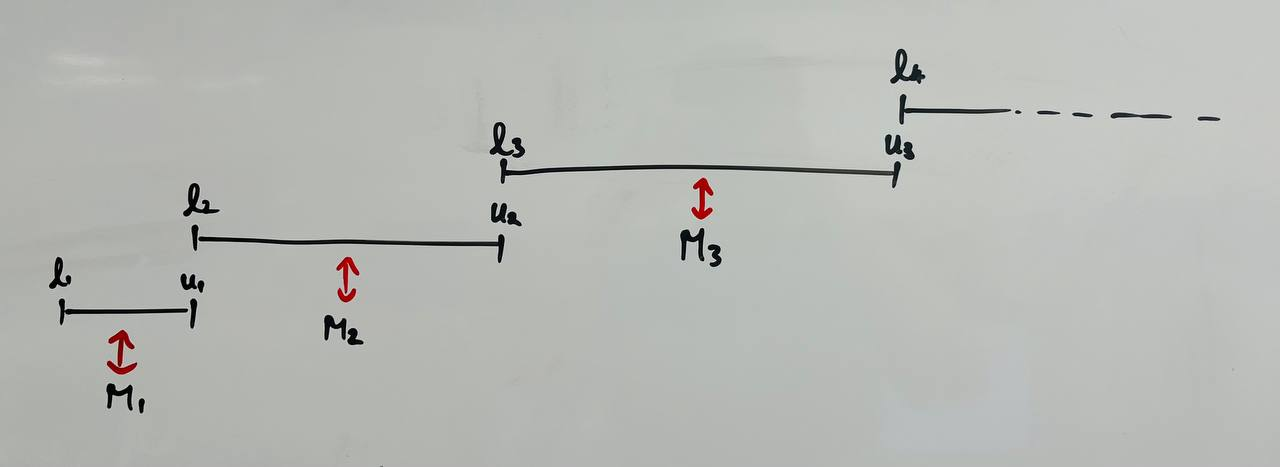
\includegraphics[width=0.65\textwidth]{media/turing_machine_intervals.jpg}
  \end{center}
  Here's where the magic happens. Consider what happens when we run $D$ on all the inputs that correspond to a single interval $I_k = (l_k, u_k]$ (thus, a single TM $M_k$). When $D$ receives the input $\texttt{1}^n$ where $n < u_k$, $D$ accepts $\texttt{1}^n$ iff $M_k$ accepts $\texttt{1}^{n + 1}$. Here, we refrain ourselves from diagonalizing. However, when $D$ receives the input $\texttt{1}^n$ where $n = u_k$, we diagonalize but on a much smaller input, i.e. $D$ accepts $\texttt{1}^n$ iff $M_k$ rejects $\texttt{1}^{l_k + 1}$. In this case, $D$ has sufficient time to simulate $M_k$ as we have established earlier. Furthermore, we have effectively demonstrated that no TM $M_k$ can accept the same language as $D$, since $D$ diverge from $M_k$ on exactly one input, i.e. on the input $\texttt{1}^n$ where $n = u_k$. To further illustrate this fact, consider the following graphical representation of an equivalence class and a non-equivalence relation that we obtain, by virtue of our construction.
  \begin{center}
    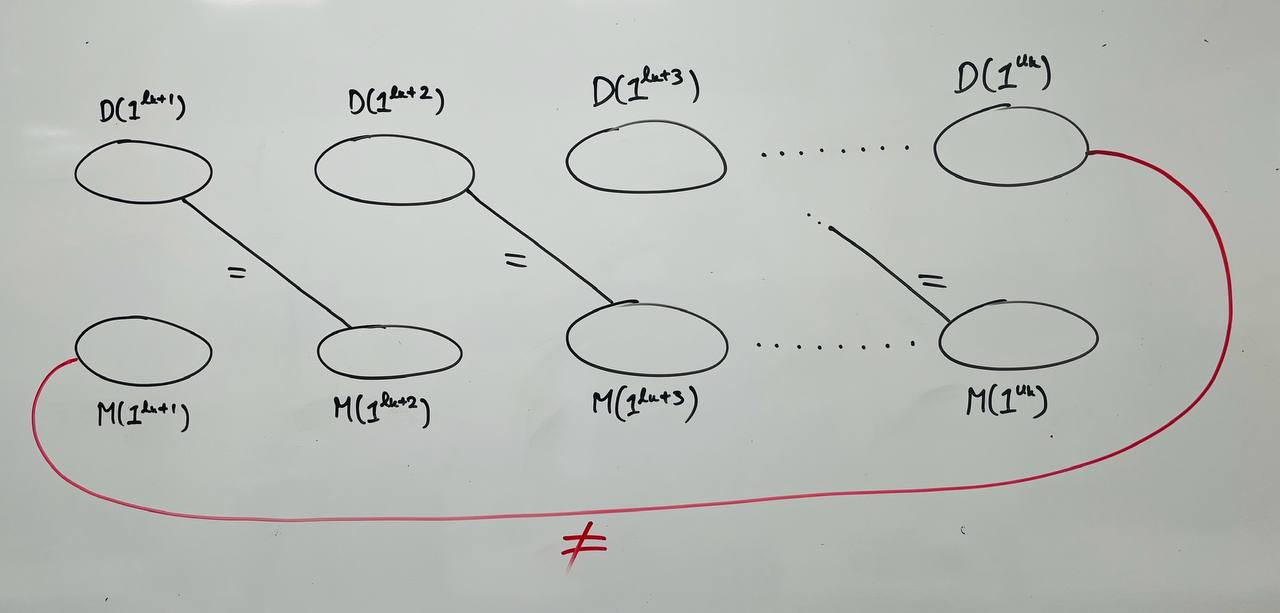
\includegraphics[width=0.75\textwidth]{media/lazy_diagonalization.jpg}
  \end{center}
  If we assume the contrary that $M_k$ accepts the same language as $D$, then we get the following new equivalence class.
  \begin{center}
    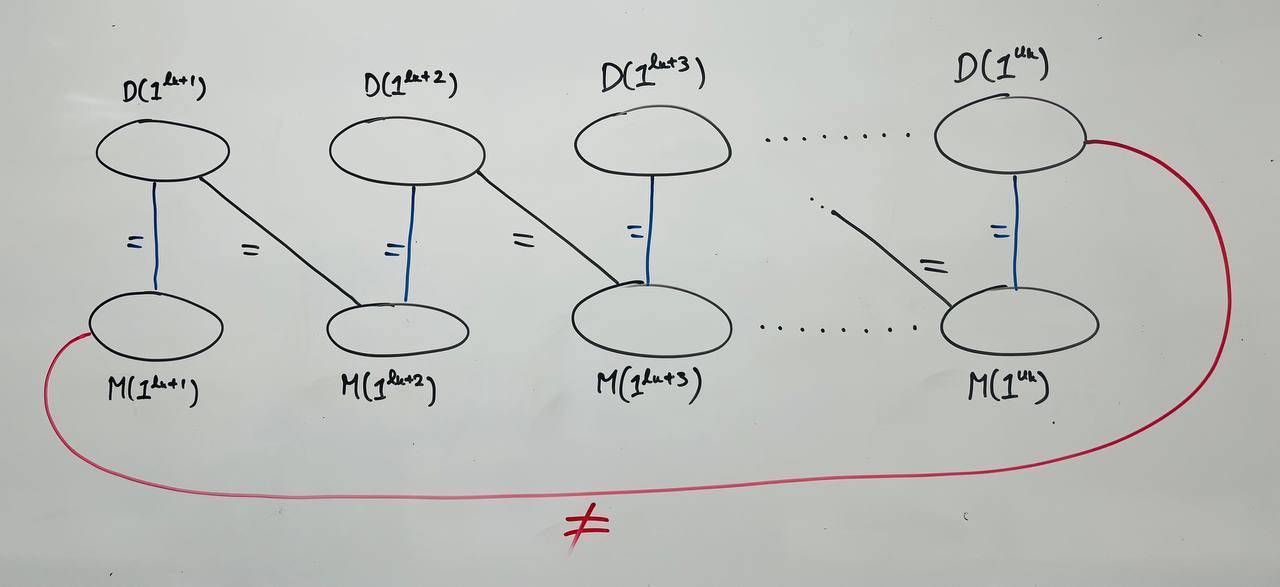
\includegraphics[width=0.75\textwidth]{media/lazy_diagonalization_contradiction.jpg}
  \end{center}
  This means that we have $M(\texttt{1}^{l_k + 1}) = D(\texttt{1}^{u_k})$ by $\relbar\!\relbar\!\relbar$ and \textcolor{blue}{$\relbar\!\relbar\!\relbar$}, but $M(\texttt{1}^{l_k + 1}) \neq D(\texttt{1}^{u_k})$ by \textcolor{red}{$\relbar\!\relbar\!\relbar$}. A contradiction.

  One last technical point. Just as in the proof of the deterministic time hierarchy theorem, we may encounter a similar issue where the asymptotic behavior of $f$ has not yet taken effect. To fix this problem, it suffices to simply restrict the simulation of $D$ on sufficiently long inputs. We then associate the first(s) of these inputs to the first interval, $I_1$.
\end{proofidea}

Now, we describe the proof formally.

\begin{proof}
  We know that the set of all Turing machines is enumerable. Let $M_k$ be the $k$-th Turing machine in the enumeration. We associate $M_k$ with an interval $I_k = (l_k, u_k]$, where $f(u_k) > 2^{f(l_k + 1)^2}$. These intervals should be disjoint but contiguous. Because $f(n + 1)$ is $o(g(n))$, some constant $n_0$ exists where $d \cdot f(n + 1) < g(n)$ for all $n \geq n_0$. We set the lower bound of the first interval, $l_1$, to $f(n_0)$. Our NTM $D$ will try to ``flip the answer'' of $M_k$ only on one input in the interval $I_k$. We define $D$ as follows:
  \begin{align*}
    D = & \ \text{``On input $w$:} \\
    & \ \quad \text{1. } \text{Let $n$ be the length of $w$.} \\
    & \ \quad \text{2. } \text{If $w$ is not of the form $\texttt{1}^n$ where $n \geq n_0$, \emph{reject}.} \\
    & \ \quad \text{3. } \text{Compute $k$ such that $n$ lies in the interval $I_k = (l_k, u_k]$.} \\
    & \ \quad \ \quad \text{3.1. } \text{If $n < u_k$, then nondeterministically simulate $M_k$ on the input} \\
    & \ \quad \ \quad \phantom{\text{3.1. }} \text{$\texttt{1}^{n + 1}$ for up to $g(n)$ steps. If $M$ accepts, then \emph{accept}. If $M$ rejects,} \\
    & \ \quad \ \quad \phantom{\text{3.1. }} \text{then \emph{reject}. (Observe that here we are \emph{not} diagonalizing.)} \\
    & \ \quad \ \quad \text{3.2. } \text{If $n = u_k$, then deterministically decide if $M_k$ accepts the input} \\
    & \ \quad \ \quad \phantom{\text{3.2. }} \text{$\texttt{1}^{l_k + 1}$ by simulating all computation paths, for up to $g(n)$ steps in} \\
    & \ \quad \ \quad \phantom{\text{3.2. }} \text{total. If $M$ accepts, then \emph{reject}. If $M$ rejects, then \emph{accept}. (Observe} \\
      & \ \quad \ \quad \phantom{\text{3.2. }} \text{that here we are indeed diagonalizing. But we are doing it on a} \\
    & \ \quad \ \quad \phantom{\text{3.2. }} \text{much shorter input than the input to $D$.)''}
  \end{align*}
  Let's analyze the running time of each stage of $D$. Stage 1 and 2 clearly operate in $O(g(n))$ time. Stage 3 can also be performed in $O(g(n))$ time, since $k \ll n$. In stage 3.1, $D$ nondeterministically simulates $M_k$ on the input $\texttt{1}^{n + 1}$. If $M_k$ really runs within $O(f(n + 1))$ time, then $D$ has sufficient time for the simulation, since $f(n + 1) = o(g(n))$. Otherwise, if $M_k$ doesn't halt, $D$ will terminate the simulation after $g(n)$ steps. In both cases, $D$ runs within $O(g(n))$ time. In stage 3.2, $D$ deterministically simulates every computation path of $M_k$ on the input $\texttt{1}^{l_k + 1}$. If $M_k$ really runs within $O(f(l_k + 1))$, $D$ again has sufficient time for the simulation. The deterministic simulation of each computation path requires $O(f(l_k + 1) \log f(l_k + 1))$, leading to a total time for all paths of $2^{O(f(l_k + 1) \log f(l_k + 1))}$. This is less than $2^{f(l_k + 1)^2} < f(u_k) = f(n) = o(g(n))$. Otherwise, if $M_k$ doesn't halt, $D$ will stop the simulation after $g(n)$ steps. In both cases, $D$ runs within $O(g(n))$ time.

  Now, we show that $A$ is not decidable in $O(f(n))$ time. Assume the contrary that some TM $M_k$ decides $A$ in time $f(n)$, where $f(n + 1)$ is $o(g(n))$. Here, $D$ can simulate $M_k$, using time $d \cdot g(n)$ for some constant $d$. The simulation will run to completion as long as the asymptotic ``kicks in''. Because $f(n + 1)$ is $o(g(n))$, some constant $n_0$ exists where $d \cdot f(n + 1) < g(n)$ for all $n \geq n_0$. Therefore, $D$'s simulation of $M_k$ will run to completion as long as the input has length $n_0$ or more. Consider what happens when we run $D$ on all the inputs $\texttt{1}^n$ where $n \geq n_0$, such that all these inputs correspond to the interval $I_k = (l_k, u_k]$. Stages 3.1 and 3.2 of $D$ ensure, respectively, that:
  \begin{align}
    \text{$M_k(\texttt{1}^{n + 1}) = D(\texttt{1}^n)$} & \qquad \text{if $l_k < n < u_k$} \\
    \text{$M_k(\texttt{1}^{l_k + 1}) \neq D(\texttt{1}^{u_k}) = D(\texttt{1}^n)$} & \qquad \text{if $n = u_k$}
  \end{align}
  By our assumption, $D$ and $M_k$ agree on all inputs $\texttt{1}^n$ in the interval $I_k = (l_k, u_k]$. Together with (2.1), this implies $M(\texttt{1}^{l_k + 1}) = D(\texttt{1}^{l_k + 1}) = M(\texttt{1}^{l_k + 2}) = D(\texttt{1}^{l_k + 2}) = \dots = M(\texttt{1}^{u_k - 1}) = D(\texttt{1}^{u_k - 1}) = M(\texttt{1}^{u_k}) = D(\texttt{1}^{u_k})$. This contradicts $M(\texttt{1}^{l_k + 1}) \neq D(\texttt{1}^{u_k})$ in (2.2). Hence, we conclude that $A$ cannot be decided in $O(f(n))$ time.
\end{proof}

\begin{remark}
  Notice that the $1 / \log f(n)$ factor does not appear in our hierarchy theorem, unlike in its deterministic counterpart. This absence is due to the efficient simulation of an NTM by another NTM, which only incurs a constant factor to the time complexity (see Exercise 2.6 of Arora and Barak \cite{arora2009computational}).
\end{remark}

\begin{remark}
  What about the term ``$+ 1$'' in $f(n + 1)$, where does it come from? This overhead arises from the fact that we have to simulate a longer input most of the time. That is, when we receive the input $\texttt{1}^{n}$, we often simulate $\texttt{1}^{n + 1}$ on $M_k$. We require that $D$ has sufficient time to simulate $M_k$, so we need $f(n + 1)$ to be $o(g(n))$.
\end{remark}

\begin{remark}
  In other literature, one would often find that a rapidly growing function $h : \NN \to \NN$ is introduced in the proof. For instance, in Arora and Barak \cite{arora2009computational}, the function $h$ is defined as follows:
  \begin{align*}
    h(n) =
    \begin{cases}
      2 & \text{if $n = 1$} \\
      2^{h(n - 1)^{1.2}} & \text{otherwise}
    \end{cases}
  \end{align*}
  The interval $I_k$ is then defined as $(l_k, u_k]$ where $l_k = h(k)$ and $u_k = h(k + 1)$. It's important to note that such a proof only works for specific instances of the theorem, e.g. proving that $\NTIME(n) \subsetneq \NTIME(n^{1.5})$. For the proof to work in the general case, we must define $h$ in relation to $f$, as demonstrated in our proof.
\end{remark}

Next, let us present a different proof due to Fortnow and Santhanam \cite{fortnow2011robust}.

\begin{proofidea}
  Once again, we define a language $A$ by describing a machine $D$ that decides it. We begin with an input $w$ of the form $\enc{M}\texttt{0}\texttt{1}^k\texttt{0}$, where $k$ is sufficiently large. How large? Well, large enough such that the sequence of $\texttt{1}$s acts as a padding, allowing the asymptotic behavior to ``kick in''. Just like in our previous proof, we use $D$ to simulate some TM $M$. Most of the time, we want to ``feed'' $M$ with a slightly longer input. If we receive $\enc{M}\texttt{0}\texttt{1}^k\texttt{0}$ for instance, we simulate $M$ on the inputs $\enc{M}\texttt{0}\texttt{1}^{k}\texttt{0}\texttt{0}$ and $\enc{M}\texttt{0}\texttt{1}^{k}\texttt{0}\texttt{1}$. We're not in a rush to diagonalize here, so $D$ will only accept if $M$ accepts on both of those inputs. We can generalize this idea: for an input of the form $\enc{M}\texttt{0}\texttt{1}^{k}\texttt{0}y$ where $y = (\texttt{0} + \texttt{1})^\ast$, we simulate $M$ on $\enc{M}\texttt{0}\texttt{1}^{k}\texttt{0}y\texttt{0}$ and $\enc{M}\texttt{0}\texttt{1}^{k}\texttt{0}y\texttt{1}$. We continue this process, by simulating $M$ on longer and longer inputs, until we reach an input $\enc{M}\texttt{0}\texttt{1}^k\texttt{0}\texttt{y}$ such that $y$ is ``long enough''. Once $y$ is long enough, instead of continuing to simulate longer inputs, we switch to simulating our initial, shorter input $\enc{M}\texttt{0}\texttt{1}^k\texttt{0}$, using $y$ as advice—basically, treating it as the nondeterministic choices. Then, we diagonalize, so $D$ accepts $\enc{M}\texttt{0}\texttt{1}^k\texttt{0}y$ iff $M$ rejects $\enc{M}\texttt{0}\texttt{1}^k\texttt{0}$ with $y$ as advice.

  Finally, we finish with the standard \textit{reductio ad absurdum} (i.e. proof by contradiction) arguments. To make this work, the advice $y$ must be long enough to simulate the longest computation path of $M$. Thus, it suffices to set the constraint $y \geq g(\len{\enc{M}} + k + 2)$ as a prerequisite for the diagonalization. At the end, we will discover that $\enc{M}\texttt{0}\texttt{1}^k\texttt{0} \in A$ iff $M$ rejects $\enc{M}\texttt{0}\texttt{1}^k\texttt{0}$ on all computation paths. But $M$ is supposed to decide $A$. This is a contradiction.
\end{proofidea}

Now, we lay out the proof more formally. To make things clearer, instead of using our original encoding of the input, i.e. $\enc{M}\texttt{0}\texttt{1}^k\texttt{0}y$, we'll rewrite it in a more mathematical way such as $(M, \texttt{1}^k, y)$. This should help make the proof easier to follow.

\begin{proof}
  The following $O(g(n))$ time NTM $D$ decides a language $A$ that is not decidable in $O(f(n))$ time.
  \begin{align*}
    D = & \ \text{``On input $w = (M, \texttt{1}^k, y)$:} \\
    & \ \quad \text{1. } \text{Let $n$ be the length of $w$.} \\
    & \ \quad \text{2. } \text{If $\len{y} < g(\len{M} + k)$ then simulate $M(M, \texttt{1}^k, y\texttt{0})$ and $M(M, \texttt{1}^k, y\texttt{1})$} \\
    & \ \quad \phantom{\text{2. }} \text{for at most $g(n)$ steps each, and \emph{accept} iff they both accept.} \\
    & \ \quad \text{3. } \text{If $\len{y} \geq g(\len{M} + k)$ then \emph{accept} iff $M(M, \texttt{1}^k, \epsilon)$ rejects using $y$ as} \\
    & \ \quad \phantom{\text{3. }} \text{advice (i.e. nondeterministic choices). Note that if $M$ does not} \\
    & \ \quad \phantom{\text{3. }} \text{halt on this computation path (e.g. because $y$ is not long enough),} \\
    & \ \quad \phantom{\text{3. }} \text{then \emph{reject}.''}
  \end{align*}
  It is easy to see that $D$ runs within $O(g(n))$ time. Now, we show that $A$ is not decidable in $O(f(n))$ time. Assume the contrary that some NTM $M_A$ decides $A$ in $O(f(n))$ time. Consider an input of the form $w = (M_A, \texttt{1}^k, \epsilon)$ for sufficiently large $k$. We have:
  \begin{align*}
    w \in A \iff & (M_A, \texttt{1}^k, \epsilon) \in A && \text{(because $w = (M_A, \texttt{1}^k, \epsilon)$)} \\
    \iff & M_A(M_A, \texttt{1}^k, \texttt{0}) = M_A(M_A, \texttt{1}^k, \texttt{1}) = 1 && \text{(by definition of $D$, stage 2)} \\
    \iff & (M_A, \texttt{1}^k, \texttt{0}), (M_A, \texttt{1}^k, \texttt{1}) \in A && \text{(because $M_A$ decides $A$)} \\
    \iff & M_A(M_A, \texttt{1}^k, \texttt{0}\texttt{0}) = M_A(M_A, \texttt{1}^k, \texttt{0}\texttt{1}) = 1 \\
    & M_A(M_A, \texttt{1}^k, \texttt{1}\texttt{0}) = M_A(M_A, \texttt{1}^k, \texttt{1}\texttt{1}) = 1 && \text{(by definition of $D$, stage 2)}
  \end{align*}
  Let $t$ be the smallest integer such that $t \geq g(\len{M_A} + k)$. Continuing the above line of reasoning we get:
  \begin{align*}
    w \in A \iff & \forall y \in \set{\texttt{0}, \texttt{1}}^t : M_A(M_A, \texttt{1}^k, y) = 1 && \text{(by induction)} \\
    \iff & \forall y \in \set{\texttt{0}, \texttt{1}}^t : (M_A, \texttt{1}^k, y) \in A && \text{(because $M_A$ decides $A$)} \\
    \iff & \forall y \in \set{\texttt{0}, \texttt{1}}^t : D(M_A, \texttt{1}^k, y) = 1 && \text{(because $D$ decides $A$)} \\
    \iff & \forall y \in \set{\texttt{0}, \texttt{1}}^t : \text{$M_A(M_A, \texttt{1}^k, \epsilon)$ rejects} \\
    & \phantom{\forall y \in \set{\texttt{0}, \texttt{1}}^t :} \ \text{on computation path $y$} && \text{(by definition of $D$, stage 3)} \\
    \iff & M_A(M_A, \texttt{1}^k, \epsilon) = 0 && \text{(by the reject condition of NTMs)} \\
    \iff & (M_A, \texttt{1}^k, \epsilon) \notin A && \text{(because $M_D$ decides $A$)} \\
    \iff & w \notin A && \text{(because $w = (M_A, \texttt{1}^k, \epsilon)$)}
  \end{align*}
  A contradiction. We conclude that no such $M_A$ can exist.
\end{proof}

\begin{remark}
  One advantage of this proof over Žák's is that we don't need to define a rapidly growing function. Also note that we only need $f(n)$ steps for the diagonalization instead of exponential in $f(n)$. However, one drawback is that it's more difficult to generalize this proof to a broader set of complexity measures.
\end{remark}

\section{Ladner's Theorem: Existence of $\NPTIME$-Intermediate Problems}
\seclabel{ladner-theorem}

\section{Oracle Machines and the Limits of Diagonalization}
\seclabel{oracle-machines-and-the-limits-of-diagonalization}

\printbibliography[nottype=image]

\end{document}
